\documentclass[a4paper,11pt]{article}

\usepackage{amsmath,amssymb,amsthm}
\usepackage[scale=0.75]{geometry}
\usepackage{graphicx}
\usepackage{hyperref}
\usepackage{bookmark}
\usepackage{hypcap}
\usepackage{cite}

\title{Simulating Water with Molecular Dynamics}
\author{Raúl Coterillo}

\begin{document}

\maketitle

This report is intended to provide a reasonable description of the steps I took to complete the assignments. The code for this project can be found in \href{https://github.com/rcote98/small-submission}{my GitHub repository}. The repository contains a \texttt{README.md} file with instructions on how to run the code. I ran all the simulations in my personal laptop (Ryzen 7, 16GB RAM), runnning Ubuntu 23.04 and GROMACS 2023.1.

\section{Simulation Environment Setup}

I created a cubic water box of 5nm$^3$ using the \texttt{solvate} command from GROMACS, using the water structure from the \texttt{spc216.gro} file. I then used the \texttt{pdb2gmx} to generate the corresponding topology file, using the AMBER03 force field and the TIP3P water model. I used the Particle Mesh Ewald method both for the Coulomb interactions and the van der Waals interactions, with a cutoff of 2nm. I chose this value since it was less than hald the size of the box, and the simulations took a reasonable amount of time with it.

\section{Energy Minimization}

Having generated the structure (.gro) and topology (.top) files, I used the \texttt{grompp} command to generate the binary input file for the energy minimization, which I later executed with the \texttt{mdrun} command. I used the steepest descend algorithm, setting a maximum force tolerance of 96.5 KJ/mol/nm, which is roughly requalt to the requested 0.1 eV/A, which took around 120 steps to converge. Figure \ref{fig:emin-equi} shows the evolution of the potential energy, and the maximum force of the system during the energy minimization.

\begin{figure}[ht]
    \centering
    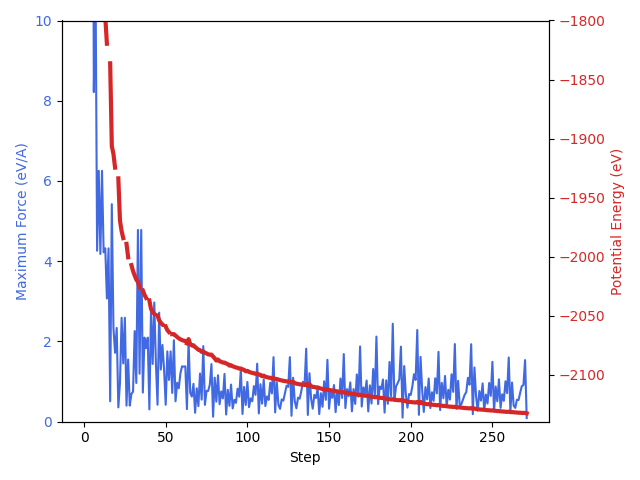
\includegraphics[width=0.49\textwidth]{../figures/emin.png} 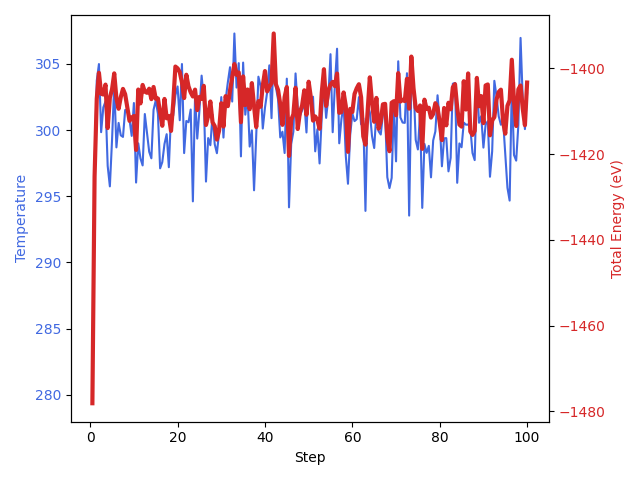
\includegraphics[width=0.49\textwidth]{../figures/equi.png}
    \caption{Evolution of the potential energy, and the maximum force of the system during the energy minimization (left) and evolution of the temperature and total energy of the system the equilibration run (right).}
    \label{fig:emin-equi}
\end{figure}

\section{Equilibration}

Using the output of the energy minimization, I used the \texttt{grompp} and \texttt{mdrun} commands again to run the equilibration simulation. I used the leap-frog algorithm for 200.000 steps with a time step of 0.5 fs, for a total of 100 ps. I used a velocity-rescale thermostat with a time constant of 0.1 ps and a temperature of 300 K. In my system, this run took 22 minutes to complete. I obtained the temperature and energies using the \texttt{energy} command in order to verify the equilibration was complete. These can be seen in Figure \ref{fig:emin-equi}.

\section{Production Run}

Finally, I used the \texttt{grompp} and \texttt{mdrun} commands again to run the production simulation, continuing the end of the equilibration run by using the \texttt{state.cpt} file. I used the leap-frog algorithm for 1.000.000 steps with a time step of 0.5 fs, for a total of 500 ps. I used a velocity-rescale thermostat with a time constant of 0.5 ps and a temperature of 300 K. In my system, this took around 1.5 hours to complete. I then used the \texttt{dipoles} command - which uses the ACF method - to calculate the dielectric constant of the system, yielding a value of 100.65, which is not very close to the experimental value of 78.4 \cite{dielectric}.

\section{Additional Tasks}

First, a brief disclaimer: 

In view of the suboptimal results obtained in the previous section, as well as the limited time I had available for this assignment, I decided to focus on the shortest additional tasks, while skipping the ones that required checking temperature, and density dependencies. A small Python script similar to the one used for the benchmark would suffice, but replicating the production run with different settings would take too long. Hence, I only included the radial distribution function and the simulation benchmark.

\subsection{Radial Distribution Function}

I calculated the OO radial distribution function (RDF) from the production run trajectory using the \texttt{gmx rdf} command. Settings included a bin size of 0.01 nm, and a cutoff of 1 nm. In Figure \ref{fig:additional} I compare the computed RDF with the experimental results obtained from X-ray scattering \cite{water_structure, xray_scattering}. I obtained the numerical data from the article's graph using a web-based figure extraction tool \cite{plotdigitizer}. We can see how the computed RDF matches the first peak, corresponding to the first shell of water molecules, pretty well. However, the other peaks, although present, are not as well defined. This could be due to the fact that the simulation is not long enough, or that the force field is not accurate enough, since the short-range threshold was set to 2 nm.

\subsection{Benchmarking}

I created a small script that runs a benchmark using the production settings. I measured the CPU and wall times of 1000 step runs with different number of threads. The results can be seen in Figure \ref{fig:additional}. In this case, the efficiency drops significantly when using more than 8 threads, which is half the cores in my CPU. This could be either due to the fact that the simulation is not very large - and hence the overhead of using more threads is not worth it - or that the rest of my computer is not idle, and hence the threads are not being used efficiently.

\begin{figure}[ht!]
    \centering
    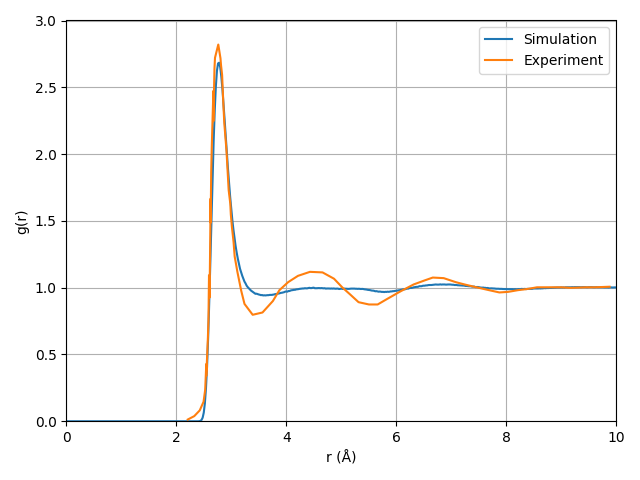
\includegraphics[width=0.49\textwidth]{../figures/rdf.png}
    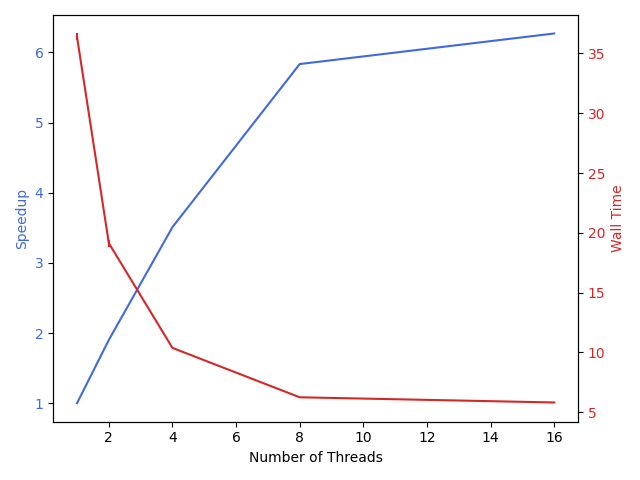
\includegraphics[width=0.49\textwidth]{../figures/bench.png}
    \caption{Comparison between computed and experimental RDFs (left) and benchmark results showing the peedup and wall times of 1000 step runs with different number of threads (right).}
    \label{fig:additional}
\end{figure}

\bibliographystyle{unsrt}
\bibliography{bibliography}

\end{document}